\chapter{Introducción}\label{ch:introduction}

Este manual operativo cubre los cuadros de instrumentos digitales \ReplicaGenOne{} y \ReplicaNextLong{} para los vehículos Volkswagen Golf~II, Jetta~II y Scirocco~II. Resume las variantes de hardware, describe sus funciones y explica cómo instalar, configurar, operar, almacenar y mantener los tableros. Las recomendaciones están dirigidas a propietarios de vehículos, electricistas automotrices y talleres que realizan la instalación del producto.

Los capítulos siguientes presentan el esquema de identificación del producto, los diagramas de pines de los conectores, las condiciones de funcionamiento y procedimientos detallados de instalación y configuración. También se incluyen referencias de mantenimiento y resolución de problemas para ambas generaciones de Replica, de modo que el cuadro pueda ser atendido sin la documentación de fábrica.

\begin{figure}[htbp]
    \centering
    \begin{subfigure}{0.48\textwidth}
        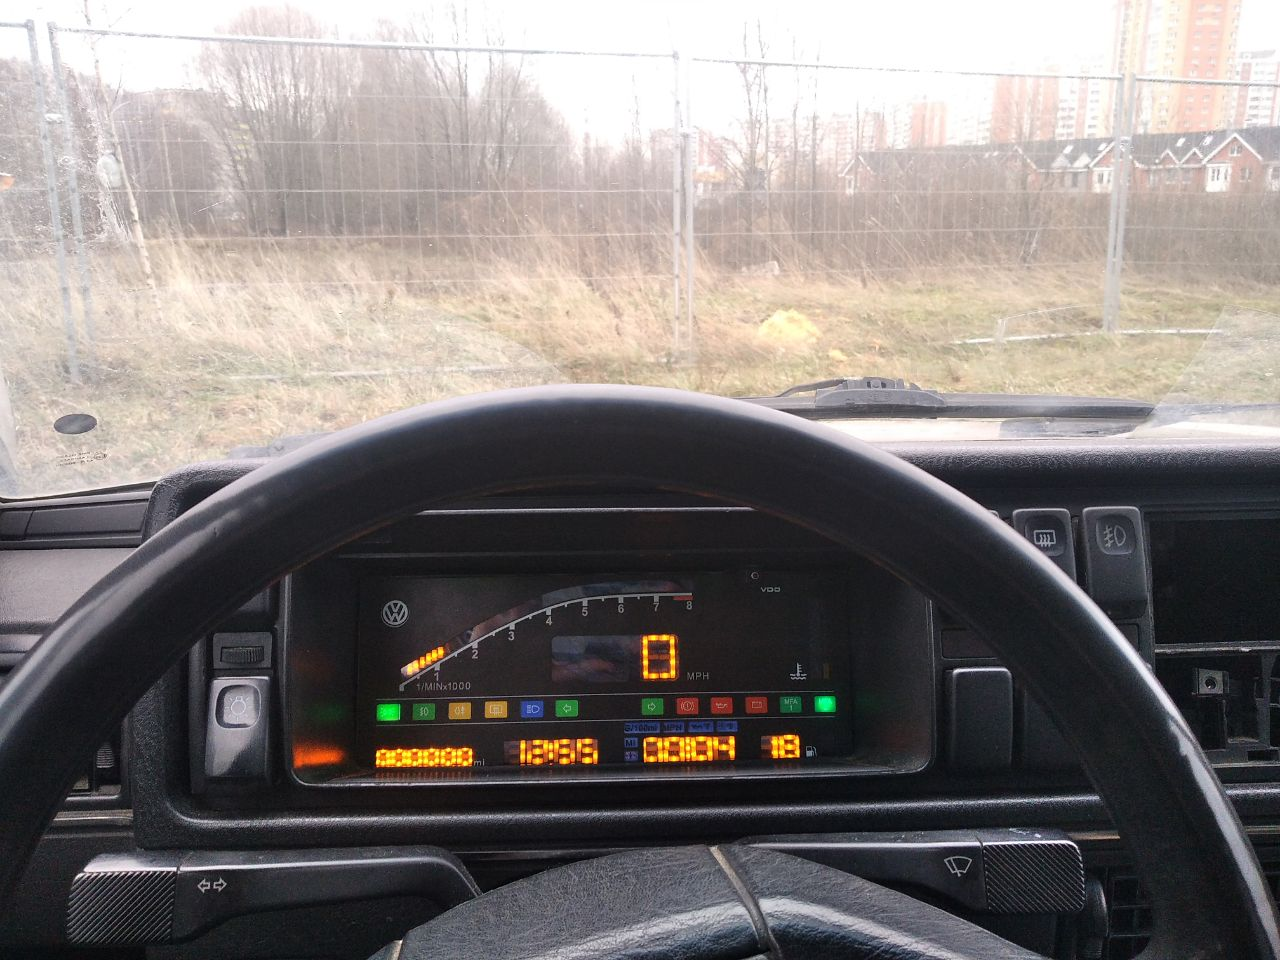
\includegraphics[width=\linewidth]{digifiz_manual/image004.jpg}
        \caption{Delivery set for the GART~8--MGF configuration.}
    \end{subfigure}\hfill
    \begin{subfigure}{0.48\textwidth}
        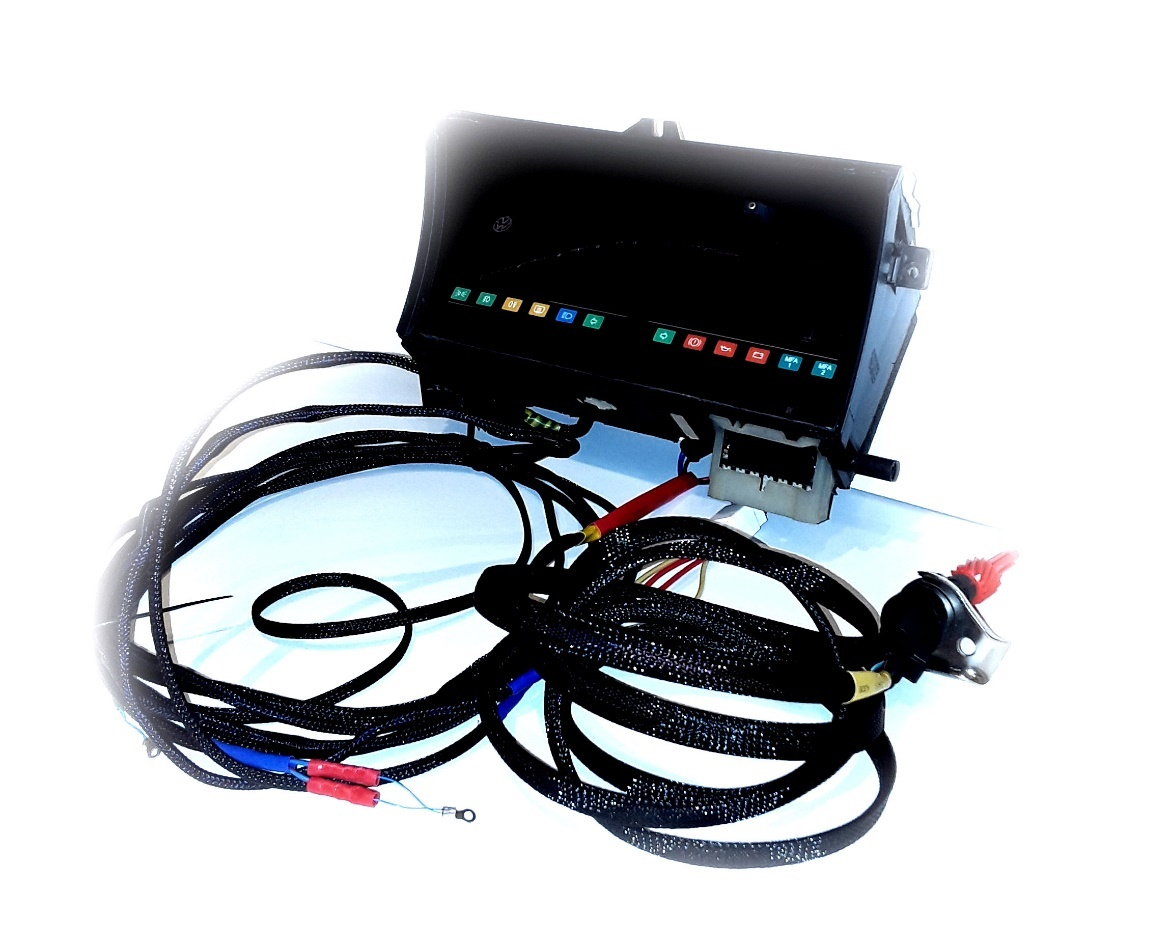
\includegraphics[width=\linewidth]{digifiz_manual/image005.jpg}
        \caption{Typical contents of a GART package.}
    \end{subfigure}
    \begin{subfigure}{0.48\textwidth}
        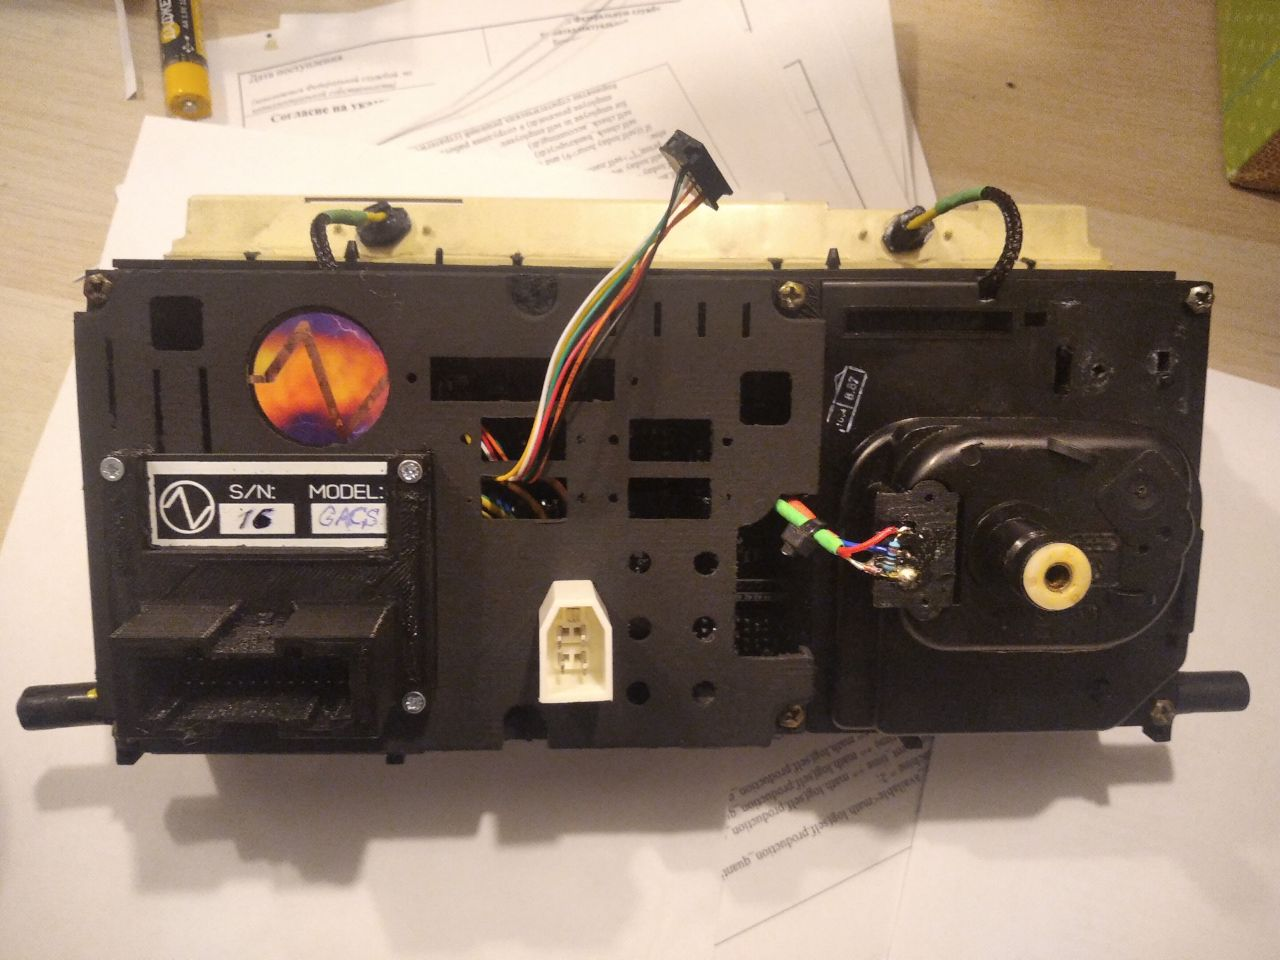
\includegraphics[width=\linewidth]{digifiz_manual/image006.jpg}
        \caption{Rear view of the single-connector GACS assembly.}
    \end{subfigure}\hfill
    \begin{subfigure}{0.48\textwidth}
        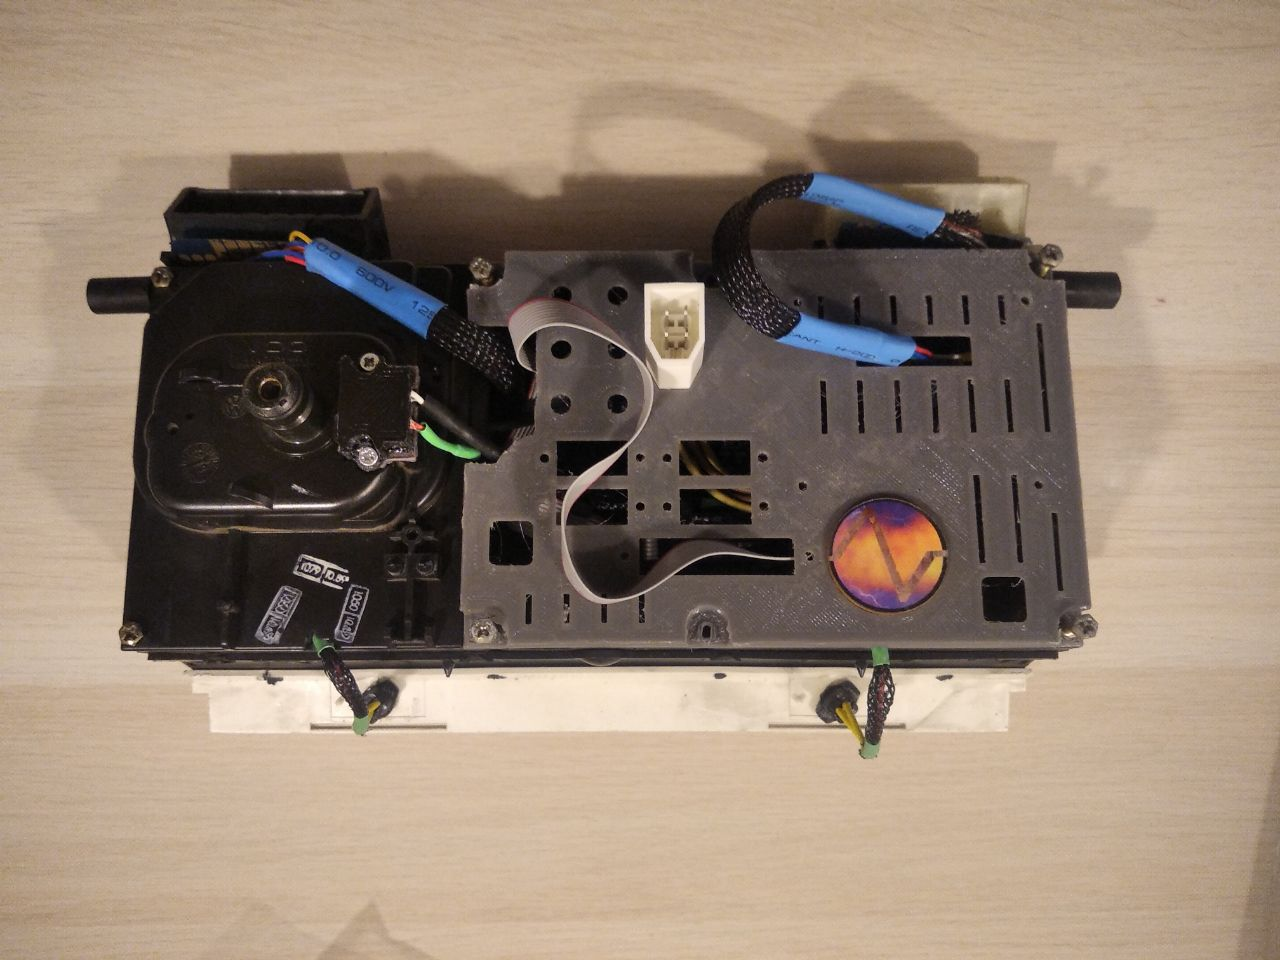
\includegraphics[width=\linewidth]{digifiz_manual/image007.jpg}
        \caption{Rear view of the dual-connector GACT assembly.}
    \end{subfigure}
    \caption{Cuadros \ReplicaGenOne{} y \ReplicaNextLong{} representativos suministrados con este manual.}
\end{figure}

Cada variante se entrega con los componentes necesarios para la cadena cinemática prevista, las unidades de medida y el estilo del mazo de cables. Los capítulos posteriores descifran los marcados de variante y proporcionan tablas de conectores para que el cuadro pueda integrarse de forma segura.
